\documentclass[10pt,a4paper]{article}
\usepackage{lmodern}
\usepackage{amssymb,amsmath}
\usepackage{ifxetex,ifluatex}
\usepackage{fixltx2e} % provides \textsubscript
\ifnum 0\ifxetex 1\fi\ifluatex 1\fi=0 % if pdftex
  \usepackage[T1]{fontenc}
  \usepackage[utf8]{inputenc}
\else % if luatex or xelatex
  \ifxetex
    \usepackage{mathspec}
    \usepackage{xltxtra,xunicode}
  \else
    \usepackage{fontspec}
  \fi
  \defaultfontfeatures{Mapping=tex-text,Scale=MatchLowercase}
  \newcommand{\euro}{€}
\fi
% use upquote if available, for straight quotes in verbatim environments
\IfFileExists{upquote.sty}{\usepackage{upquote}}{}
% use microtype if available
\IfFileExists{microtype.sty}{%
\usepackage{microtype}
\UseMicrotypeSet[protrusion]{basicmath} % disable protrusion for tt fonts
}{}
\usepackage{color}
\usepackage{fancyvrb}
\newcommand{\VerbBar}{|}
\newcommand{\VERB}{\Verb[commandchars=\\\{\}]}
\DefineVerbatimEnvironment{Highlighting}{Verbatim}{commandchars=\\\{\}}
% Add ',fontsize=\small' for more characters per line
\usepackage{framed}
\definecolor{shadecolor}{RGB}{248,248,248}
\newenvironment{Shaded}{\begin{snugshade}}{\end{snugshade}}
\newcommand{\AlertTok}[1]{\textcolor[rgb]{0.94,0.16,0.16}{#1}}
\newcommand{\AnnotationTok}[1]{\textcolor[rgb]{0.56,0.35,0.01}{\textbf{\textit{#1}}}}
\newcommand{\AttributeTok}[1]{\textcolor[rgb]{0.77,0.63,0.00}{#1}}
\newcommand{\BaseNTok}[1]{\textcolor[rgb]{0.00,0.00,0.81}{#1}}
\newcommand{\BuiltInTok}[1]{#1}
\newcommand{\CharTok}[1]{\textcolor[rgb]{0.31,0.60,0.02}{#1}}
\newcommand{\CommentTok}[1]{\textcolor[rgb]{0.56,0.35,0.01}{\textit{#1}}}
\newcommand{\CommentVarTok}[1]{\textcolor[rgb]{0.56,0.35,0.01}{\textbf{\textit{#1}}}}
\newcommand{\ConstantTok}[1]{\textcolor[rgb]{0.00,0.00,0.00}{#1}}
\newcommand{\ControlFlowTok}[1]{\textcolor[rgb]{0.13,0.29,0.53}{\textbf{#1}}}
\newcommand{\DataTypeTok}[1]{\textcolor[rgb]{0.13,0.29,0.53}{#1}}
\newcommand{\DecValTok}[1]{\textcolor[rgb]{0.00,0.00,0.81}{#1}}
\newcommand{\DocumentationTok}[1]{\textcolor[rgb]{0.56,0.35,0.01}{\textbf{\textit{#1}}}}
\newcommand{\ErrorTok}[1]{\textcolor[rgb]{0.64,0.00,0.00}{\textbf{#1}}}
\newcommand{\ExtensionTok}[1]{#1}
\newcommand{\FloatTok}[1]{\textcolor[rgb]{0.00,0.00,0.81}{#1}}
\newcommand{\FunctionTok}[1]{\textcolor[rgb]{0.00,0.00,0.00}{#1}}
\newcommand{\ImportTok}[1]{#1}
\newcommand{\InformationTok}[1]{\textcolor[rgb]{0.56,0.35,0.01}{\textbf{\textit{#1}}}}
\newcommand{\KeywordTok}[1]{\textcolor[rgb]{0.13,0.29,0.53}{\textbf{#1}}}
\newcommand{\NormalTok}[1]{#1}
\newcommand{\OperatorTok}[1]{\textcolor[rgb]{0.81,0.36,0.00}{\textbf{#1}}}
\newcommand{\OtherTok}[1]{\textcolor[rgb]{0.56,0.35,0.01}{#1}}
\newcommand{\PreprocessorTok}[1]{\textcolor[rgb]{0.56,0.35,0.01}{\textit{#1}}}
\newcommand{\RegionMarkerTok}[1]{#1}
\newcommand{\SpecialCharTok}[1]{\textcolor[rgb]{0.00,0.00,0.00}{#1}}
\newcommand{\SpecialStringTok}[1]{\textcolor[rgb]{0.31,0.60,0.02}{#1}}
\newcommand{\StringTok}[1]{\textcolor[rgb]{0.31,0.60,0.02}{#1}}
\newcommand{\VariableTok}[1]{\textcolor[rgb]{0.00,0.00,0.00}{#1}}
\newcommand{\VerbatimStringTok}[1]{\textcolor[rgb]{0.31,0.60,0.02}{#1}}
\newcommand{\WarningTok}[1]{\textcolor[rgb]{0.56,0.35,0.01}{\textbf{\textit{#1}}}}
\usepackage{longtable,booktabs}
\ifxetex
  \usepackage[setpagesize=false, % page size defined by xetex
              unicode=false, % unicode breaks when used with xetex
              xetex]{hyperref}
\else
  \usepackage[unicode=true]{hyperref}
\fi
\hypersetup{breaklinks=true,
            bookmarks=true,
            pdfauthor={},
            pdftitle={titre non affiche},
            colorlinks=true,
            citecolor=blue,
            urlcolor=blue,
            linkcolor=magenta,
            pdfborder={0 0 0}}
\urlstyle{same}  % don't use monospace font for urls
\setlength{\parindent}{0pt}
\setlength{\parskip}{6pt plus 2pt minus 1pt}
\setlength{\emergencystretch}{3em}  % prevent overfull lines
\setcounter{secnumdepth}{5}

\providecommand{\tightlist}{%
  %\setlength{\itemsep}{0pt}
  \setlength{\parskip}{0pt}
  }

%%% Use protect on footnotes to avoid problems with footnotes in titles
\let\rmarkdownfootnote\footnote%
\def\footnote{\protect\rmarkdownfootnote}


  \title{titre non affiche}
    \author{}
    \date{}
  
% Packages

\usepackage[utf8]{inputenc}
\usepackage{setspace}
%\usepackage[french]{babel} % Pour la traduction française
%\renewcommand\frenchtablename{\textsc{Tableau}} %renommer table en tableau
%\AtBeginDocument{\renewcommand{\abstractname}{Synthèse}} %titre abstract
\usepackage{mathptmx} %times roman {mathptmx} OU {newtxtext} 
\DeclareSymbolFont{calletters}{OMS}{cmsy}{m}{n}  %pour differencier mathcal et mathscr
\DeclareSymbolFontAlphabet{\mathcal}{calletters} %pour differencier mathcal et mathscr
\usepackage[hmargin=1.5cm,vmargin=1.5cm]{geometry} % marges
\usepackage{caption}
\usepackage{graphicx}
\usepackage{natbib}
\usepackage[dvipsnames]{xcolor}
\usepackage{fontawesome5}
\DeclareMathOperator{\arctanh}{arctanh}
\usepackage{amsfonts}
\usepackage{dsfont}
\usepackage{xspace}
\usepackage{enumitem}
\usepackage{pifont}
\usepackage{wrapfig}
\usepackage{textpos}
\usepackage{array}
\usepackage{amsmath}
\usepackage{mathrsfs}  
\usepackage{tcolorbox}
\usepackage{here} %positionner les images
\usepackage{colortbl} %colorer un tableau
\usepackage[normalem]{ulem} %sout

\usepackage{ntheorem}
\theoremstyle{break}
\newtheorem{theorem}{Théorème}[section]
\newtheorem{lemma}{Lemme}[section]
\newtheorem{proposition}{Propriété}[section]
\newtheorem{corollary}{Corollaire}[section]
\newenvironment{proof}{\textbf{Preuve}}{$\Box$}
\newtheorem{definition}{Définition}[section]
\newtheorem{example}{Exemple}[section]
\newtheorem{remark}{Remarque}[section]
\newtheorem{conjecture}{Hypothèse}[section]
\newtheorem{problem}{Problème}[section]
\newtheorem{algo}{Algorithme}[section]
\def\cP{{\mathcal{P}}} 
\def\cM{{\mathcal{M}}} 
\def\CC{{\mathcal{C}}} 
\def\NN{{\mathbb{N}}}
\def\RR{{\mathbb{RR}}}
\definecolor{rougeENSAE}{RGB}{188, 24, 39}

%\onehalfspacing 



% % Page de garde
% 
% \makeatletter
% \def\@maketitle{%
%   \clearpage
%  \thispagestyle{empty}
% 
% \begin{textblock*}{\textwidth}(-7cm,-3.5cm)
% \begin{center}
% \includegraphics[height=3cm]{img/900px-LOGO-ENSAE.png}
% \end{center}
% \end{textblock*}
% 
% \begin{minipage}{0.3\textwidth}
%   \begin{flushleft} \large
%     \textbf{ANTUNEZ Kim \vspace{8.75mm} }
%   \end{flushleft}
% \end{minipage}
% \begin{minipage}{0.6\textwidth}
%   \begin{flushright} 
%   \large{
%     \textbf{ENSAE 2\up{ème} année\\}
%   }     
%   \small
%     \textbf{ 
%         \textit{Stage d'application\\
%         Année scolaire 2019 - 2020}
%     }
%   \end{flushright}
% \end{minipage}
% 
% \vspace*{2cm}
% 
% \begin{center}
%     \fbox{\parbox{0.9\textwidth}{
%         \begin{huge}\begin{center}
%             \textbf{Échantillonnage spatial déterminantal}\\
%         \end{center}\end{huge}}}
% \end{center}
% 
% \vfill
% 
% \begin{center}
% \includegraphics[width=0.6\linewidth]{img/markdown-figPG-1}
% \end{center}
% 
% \vfill
%     
% \begin{minipage}{0.4\textwidth}
%     \begin{flushleft} \large 
%     \textbf{Direction générale de l'Insee\\
%         Montrouge, France
%     }
%   \end{flushleft}
% \end{minipage} 
% \begin{minipage}{0.6\textwidth}
%   \begin{flushright} \large
%     \textbf{
%         Maître de stage : Vincent \textsc{Loonis}\\
%         08/06/2020 - 14/08/2020
%     }
%   \end{flushright}
% \end{minipage}    
% 
% \vspace*{1cm}
% 
% 
% \textcolor{rougeENSAE}{\rule{10mm}{1.5mm}}
% 
% \scriptsize
% \textbf{ENSAE Paris}\newline TSA 26644
% \rightline{\href{www.ensae.fr}{\textcolor{rougeENSAE}{\textbf{www.ensae.fr}}}$\quad \qquad \qquad$}
% Service des relations entreprises et des stages\newline
% 5, avenue Henry Le Chatelier -- 91764 PALAISEAU CEDEX -- FRANCE -- Tél : +33 (0)1 70 26 67 39 -- Courriel : stage\symbol{64}ensae.fr
% 
% \normalsize
% 
% \clearpage
% \setcounter{page}{1} %ne pas numéroter le sommaire: mettre 0
% \onehalfspacing
% 
% }
% 
% \makeatother% cinsérer page de garde

% Environnement colonnes

\newenvironment{cols}[1][]{}{}

\newenvironment{col}[1]{\begin{minipage}{#1}\ignorespaces}{%
\end{minipage}
\ifhmode\unskip\fi
\aftergroup\useignorespacesandallpars}

\def\useignorespacesandallpars#1\ignorespaces\fi{%
#1\fi\ignorespacesandallpars}

\makeatletter
\def\ignorespacesandallpars{%
  \@ifnextchar\par
    {\expandafter\ignorespacesandallpars\@gobble}%
    {}%
}
\makeatother
\usepackage{subfig}


\usepackage[tikz]{bclogo}
\newcounter{comptEncadre}
\renewcommand\thecomptEncadre{%\thesection.
\arabic{comptEncadre}}
\definecolor{processblue}{cmyk}{0.96,0,0,0}
\newenvironment{encadre}[2][false]{\refstepcounter{comptEncadre}
      %\addcontentsline{exp}{encadres}{\protect\numberline{\thecomptEncadre}#1}%
\begin{bclogo}[couleur=processblue!5,arrondi=0.1,
logo=\bcloupe,barre=none,couleurBord=blue!60!green,nobreak = #1]{ {\sc \textbf{Encadré \thecomptEncadre}} -  #2}
\smallskip
}{\end{bclogo}}


% nouvelle page de titre Kim
\usepackage{titling}
\setlength{\droptitle}{-8em}
\usepackage{lipsum}
\title{\textbf{TP3: NN and CNN with \texttt{Pytorch}} \medskip \\ \large \emph{Kim ANTUNEZ, Isabelle BERNARD (Group : Mr Denis)}}
\author{}


\renewcommand\maketitlehookc{\vspace{-10ex}}
% nouvelle page de titre Kim

%espaces entre sections Kim
\usepackage{titlesec}
\titlespacing*{\section}
{0pt}{1.5ex plus 1ex minus .2ex}{0.3ex plus .2ex}
\titlespacing*{\subsection}
{0pt}{1.5ex plus 1ex minus .2ex}{0.3ex plus .2ex}
%espaces entre sections Kim


\begin{document}

\maketitle


\vspace{-20truemm}

\hypertarget{introduction}{%
\section{Introduction}\label{introduction}}

\begin{tcolorbox}

\textbf{Question 1:} Solve the problem \(\min_{w \in \mathbb{R}^5}\, (1 - x^\top w)^2\) with \(x = (1, \ldots, 1)^\top \in \mathbb{R}^5\) analytically and compare to the result of the Gradient Descent.

\end{tcolorbox}

If \(x = (1, \ldots, 1)^\top \in \mathbb{R}^5\) and \(w = (w_1, \ldots, w_5)^\top \in \mathbb{R}^5\)

Let be \(f(w) = f(w_1, \dots w_5) = (1 - x^\top w)^2 = (1 - w_1 - w_2 - w_3 - w_4 - w_5)^2\)

As \(f\) is a positive function, we clearly see that the minimum of \(f\) is 0 and is reached for all the points w such as \(\sum_{k=1}^5 w_k = 1\)

In particular the point \(w=(0.2, 0.2, 0.2, 0.2, 0.2)\) which is the result of the previous Gradient Descent is one of the minima of the function. We can note that the result of the gradient descent would have been different if we had chosen another \(w_0 \ne (0, 0, 0, 0, 0)\)

\begin{tcolorbox}

\textbf{Question 2:} Recalling the theory of numerical optimization, what is the learning rate \texttt{lr} that we need to set to ensure the fastest convergence?

\end{tcolorbox}

The learning rate \(\eta\) is a hyperparameter that determines how fast the algorithm learns. It controls how much to change the model in response to the estimated error each time the model weights are updated following this formula : \(w_k = w_{k - 1} - \eta \nabla L(w_{k - 1})\). The learning rate is one of the most important hyperparameter when configuring our neural network. Choosing it is challenging because :

\begin{itemize}
\item
  \textbf{if \(\eta\) is too large}, the model learns too much (rapid learning) and may result in learning a sub-optimal set of weights or an unstable training process (unable to effectively gradually decrease our loss). The gradient descent can overshoot the local lowest value. It may fail to converge to a good local minimum or may even diverge.
\item
  \textbf{if \(\eta\) is too small}, the model learns too little (slow learning) and it may take too long to converge or would even get stuck and unable to converge to a good local minima
\end{itemize}

\textbf{\faArrowCircleRight{} To conclude, we must choose a learning rate which is larger enough to converge fast enough but not to large to prevent from rapid learning (being unable to converge to a good minimum). To choose it, we have to test different hyperparameters and define which is the best compromise (``hyperparameter tuning'').}

\emph{Source : \href{https://machinelearningmastery.com/understand-the-dynamics-of-learning-rate-on-deep-learning-neural-networks/}{here} and \href{https://www.deeplearningwizard.com/deep_learning/boosting_models_pytorch/lr_scheduling/}{here}}

\begin{tcolorbox}

\textbf{Question 3:} Explain the connection of \texttt{loss.backward()} and the backpropagation for feedforward neural nets.

\end{tcolorbox}

Backpropagation is a short form for ``backward propagation of errors''. Technically, the backpropagation algorithm is a method for training the weights in a multilayer feed-forward neural network. As such, it requires a network structure to be defined of one or more layers where one layer is fully connected to the next layer. A standard network structure is one input layer, one hidden layer, and one output layer.
The backpropagation computes the gradient of the loss function with respect to the weights of the network. This helps to update weights to minimize loss. There are many update rules for updating the weights : mainly Gradient descent, Stochastic gradient descent, RMSProp, Adam.

\texttt{loss.backward()} computes gradient of loss (dloss/dw) with respect to all the parameters w in loss for which \texttt{requires\_grad\ =\ True}. It stores them in the parameter.grad (\texttt{w.grad}) attribute for every parameter w.

Here, the output values are compared with the correct answer to compute the value of a predefined error-function. By various techniques, the error is then fed back through the network. Using this information, the algorithm adjusts the weights of each connection in order to reduce the value of the error function by some small amount. After repeating this process for a sufficiently large number of training cycles, the network will usually converge to some state where the error of the calculations is small. In this case, one would say that the network has learned a certain target function. To adjust weights properly, one applies a general method for non-linear optimization that is called gradient descent. For this, the network calculates the derivative of the error function with respect to the network weights, and changes the weights such that the error decreases (thus going downhill on the surface of the error function). For this reason, back-propagation can only be applied on networks with differentiable activation functions.

\emph{Source : \href{https://medium.com/analytics-vidhya/backpropagation-algorithm-using-pytorch-ee1287888aca}{here}}

\hypertarget{multi-layer-perceptron}{%
\section{Multi layer perceptron}\label{multi-layer-perceptron}}

\begin{tcolorbox}

\textbf{Question 4:} Run the above block several times. Is it plotting the same number all the time? If not, why?

\end{tcolorbox}

No, because \texttt{torch.utils.data.random\_split} randomly splits the dataset all\_train into non-overlapping new datasets (trainset and valset).
We can optionally fix the generator for reproducible results, e.g.:

\texttt{trainset,\ valset\ =\ \ torch.utils.data.random\_split(all\_train,\ {[}num\_train,\ \ len(all\_train)\ -\ num\_train{]},\ generator=torch.Generator().manual\_seed(42))}

\hypertarget{problem-1-logistic-regression-via-pytorch}{%
\section{Problem 1: Logistic regression via pytorch}\label{problem-1-logistic-regression-via-pytorch}}

\textbf{1. Mathematical description of logistic regression}

Logistic Regression can be thought of as a simple, fully-connected neural network with one hidden layer.

In the following network (see diagram), the \textbf{forward pass} are the three steps from the input to the output layer.

\begin{center}
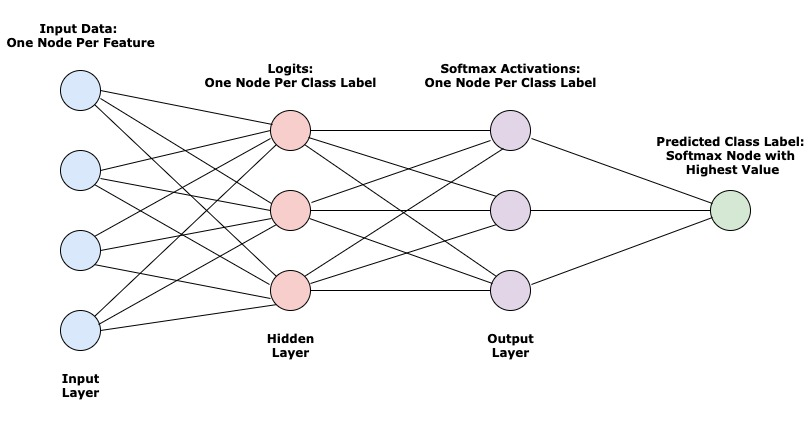
\includegraphics[width=0.8\textwidth]{img/logistic_regression_diagram.jpg}
\end{center}

\begin{enumerate}
\def\labelenumi{\arabic{enumi}.}
\tightlist
\item
  The input data in blue are the \(n\) features (\(n =4\) in the example)
\item
  In the hidden layer in red are the resulting matrix \(Z\) of multiplying each m rows (training observations) of the dataset a weight matrix with n rows and k columns, with \(k\) the number of unique classes you want to predict. We also add a bias to the result. The equation is \(Z_{[m,k]} = X_{[m,n]} W_{[n,k]} + b_{[m,k]}\). \(z_{i,j}\) is called the logit for the \(j^{th}\) label of the \(i^{th}\) training example
\end{enumerate}

\emph{Remark : To represent multinomial classes, we use \textbf{one-hot encoding} as we saw for TP2 : a simple transformation of a 1-dimensional vector of length \(m\) into a binary tensor of shape \((m, k)\), where k is the number of unique classes. Each column in the new tensor represents a specific class label and for every row there is exactly one column with a 1, everything else is zero. But the PyTorch's loss function that we use (\texttt{nn.CrossEntropyLoss}) take directly class labels as their targets so we don't need to convert targets into onehot vectors.}

\begin{enumerate}
\def\labelenumi{\arabic{enumi}.}
\setcounter{enumi}{2}
\tightlist
\item
  For the output layer in green, every logit of the matrix \(Z\) are passed through an activation function called Softmax (equation below) and the results are numbers between 0 and 1. \(a_{i,j}\) will correspond to the probability that observation \(i\) is of the type \(j\).
\end{enumerate}

\begin{equation*}
\sigma_{i}(z_{i,j}) = \frac{e^{z_{i,j}}}{\sum_{n=0}^{k}e^{z_{i,n}}} = a_{i, j}
\end{equation*}

\faArrowCircleRight{} Finally, we pick the node in the output layer that has the highest probability and choose that as the predicted class label.

\textbf{2. Mathematical description of optimization algorithm that you use}

At the end of each forward pass in the training process, we use the activations to determine the performance of the model using the cost called \textbf{Cross Entropy Loss} : \(Cross\:Entropy\:Loss = -\frac{1}{m}\sum_{i=0}^{m} \sum_{j=0}^{k} y_{i,j} \cdot \log (a_{i,j})\)

\emph{Remark : To prevent the model from overfitting, we can also regularize the regression by simply adding a term to the cost function intended to penalize model complexity. We use : \(L2\:Regularized\:Loss = -\frac{1}{m}\sum_{i=0}^{m} \sum_{j=0}^{k} y_{i,j} \cdot \log (a_{i,j}) + \lambda \sum_{i=0}^{n} \sum_{j=0}^{k} w_{i,j}^2\) with \(\lambda \leq 0\) a hyperparameter to be tuned. We don't do it here because it is not specifically asked.}

Finally, during the \textbf{backward pass}, go back through the network and make adjustments to every hidden layer's parameters. The goal is to reduce the loss in the next training iteration. In this particular case of Logistic Regression, there's only one layer of parameters that will get adjusted by a method called \textbf{Gradient Descent} :

\begin{enumerate}
\def\labelenumi{\arabic{enumi}.}
\tightlist
\item
  We first get the gradient of each model parameter using the backpropagation algorithm.
\end{enumerate}

\[\nabla (W) =
\begin{bmatrix}
\nabla (w_{0,0}) & \nabla (w_{0,1}) & \cdots & \nabla (w_{0,k}) \\
\nabla (w_{1,0}) & \nabla (w_{1,1}) & \cdots & \nabla (w_{1,k}) \\
\vdots  & \vdots  & \cdots & \vdots \\
\nabla (w_{n,0}) & \nabla (w_{n,1}) & \cdots & \nabla (w_{n,k})
\end{bmatrix} \qquad \text{where} \qquad \nabla (w_{f,l}) = 
[\frac{1}{m} \sum_{i=0}^{m} \left( x_{i,f} * (y_{i, l} - a_{i, l}) \right)] + [2 \lambda * w_{f,l}]\]

\[\nabla (b) = 
\begin{bmatrix}
\nabla (b_{0}) & \nabla (b_{1}) & \cdots & \nabla (b_{k})
\end{bmatrix} \qquad \text{where} \qquad \nabla (b_{l}) = \frac{1}{m} \sum_{i=0}^{m} \left( y_{i, l} - a_{i, l} \right)\]

\begin{enumerate}
\def\labelenumi{\arabic{enumi}.}
\setcounter{enumi}{1}
\tightlist
\item
  We update each model parameter in the opposite direction of its gradient.
\end{enumerate}

\emph{Source : \href{https://aaronkub.com/2020/02/12/logistic-regression-with-pytorch.html}{here} and \href{https://towardsdatascience.com/logistic-regression-on-mnist-with-pytorch-b048327f8d19}{here}}

\textbf{3. High level idea of how to implement logisitic regression with pytorch}

\textbf{Preliminary remark:} In the function \texttt{train} constructed by the teacher, there was a little mistake that we had to correct so that the following code works. The following line\ldots{}

\begin{verbatim}
        #careful : the following line was a mistake in the teacher's proposition ! 
        #outputs = net(inputs) # mistake we need to replace net by the parameter "model"
\end{verbatim}

had been replaced by\ldots{}

\begin{verbatim}
        outputs = model(inputs) # Forwards stage (prediction with current weights)
        
      
\end{verbatim}

\begin{Shaded}
\begin{Highlighting}[]
\CommentTok{# Add multinomial logistic regression}
\KeywordTok{class}\NormalTok{ MultinomialLogisticRegression(nn.Module):}
    \KeywordTok{def} \FunctionTok{__init__}\NormalTok{(}\VariableTok{self}\NormalTok{, input_size, output_size):}
        \BuiltInTok{super}\NormalTok{().}\FunctionTok{__init__}\NormalTok{()}
        \VariableTok{self}\NormalTok{.classifier }\OperatorTok{=}\NormalTok{ torch.nn.Linear(input_size, output_size)}
        \CommentTok{# We don't use Softmax here because the CrossEntropyLoss function computes softmax before the CE.}

    \KeywordTok{def}\NormalTok{ forward(}\VariableTok{self}\NormalTok{, x):}
\NormalTok{        x }\OperatorTok{=}\NormalTok{ x.reshape(}\OperatorTok{-}\DecValTok{1}\NormalTok{, input_size)}
\NormalTok{        x }\OperatorTok{=} \VariableTok{self}\NormalTok{.classifier(x)}
        \ControlFlowTok{return}\NormalTok{ x}
\end{Highlighting}
\end{Shaded}

\begin{Shaded}
\begin{Highlighting}[]
\CommentTok{# initializing our model/loss/optimizer}
\NormalTok{MLR }\OperatorTok{=}\NormalTok{ MultinomialLogisticRegression(input_size, output_size) }
\NormalTok{criterion }\OperatorTok{=}\NormalTok{ nn.CrossEntropyLoss() }\CommentTok{# /!\textbackslash{} computes softmax and then the cross entropy}
\NormalTok{optimizer }\OperatorTok{=}\NormalTok{ optim.SGD(MLR.parameters(), lr}\OperatorTok{=}\NormalTok{lr)}
\end{Highlighting}
\end{Shaded}

\begin{Shaded}
\begin{Highlighting}[]
\CommentTok{# num_epochs indicates the number of passes over the data}
\ControlFlowTok{for}\NormalTok{ epoch }\KeywordTok{in} \BuiltInTok{range}\NormalTok{(num_epochs):}
    
    \CommentTok{# makes one pass over the train data and updates weights}
\NormalTok{    train(MLR, trainloader, criterion, optimizer, epoch, num_epochs)}

    \CommentTok{# makes one pass over validation data and provides validation statistics}
\NormalTok{    val_loss, val_acc }\OperatorTok{=}\NormalTok{ validation(MLR, valloader, criterion)}
\end{Highlighting}
\end{Shaded}

\textbf{4. Report classification accuracy on test data.}

\textbf{\faArrowCircleRight{} The accuracy is 83 \% with 2 epochs on test data.}

\begin{Shaded}
\begin{Highlighting}[]
\CommentTok{# Let us evaluate our net on the test set that we have never seen!}
\NormalTok{testset }\OperatorTok{=}\NormalTok{ datasets.MNIST(}\StringTok{'data/'}\NormalTok{,}
\NormalTok{                         download}\OperatorTok{=}\VariableTok{True}\NormalTok{,}
\NormalTok{                         train}\OperatorTok{=}\VariableTok{False}\NormalTok{,}
\NormalTok{                         transform}\OperatorTok{=}\NormalTok{transforms.ToTensor())}
\NormalTok{testloader }\OperatorTok{=}\NormalTok{ torch.utils.data.DataLoader(testset, batch_size}\OperatorTok{=}\NormalTok{batch_size, shuffle}\OperatorTok{=}\VariableTok{True}\NormalTok{)}

\NormalTok{test_loss, test_acc }\OperatorTok{=}\NormalTok{ validation(MLR, testloader, criterion)}
\BuiltInTok{print}\NormalTok{(}\SpecialStringTok{f'Test accuracy: }\SpecialCharTok{\{}\NormalTok{test_acc}\SpecialCharTok{\}}\SpecialStringTok{'}\NormalTok{)}
\end{Highlighting}
\end{Shaded}

\begin{verbatim}
Test accuracy: 0.83
\end{verbatim}

\hypertarget{problem-2-dropout}{%
\section{Problem 2: Dropout}\label{problem-2-dropout}}

\textbf{1. High level description of the dropout}

The idea of ``Dropout'' is to prevent from overfitting in deep neural network with large parameters on the data. As you can see in the following figure, ``Dropout'' deactivates the neurons randomly at each training step instead of training the data on the original network, we train the data on the network with dropped out nodes. In the next iteration of the training step, the hidden neurons which are deactivated by dropout changes because of its probabilistic behavior. In this way, by applying dropout i.e\ldots{}deactivating certain individual nodes at random during training we can simulate an ensemble of neural network with different architectures.

\begin{center}
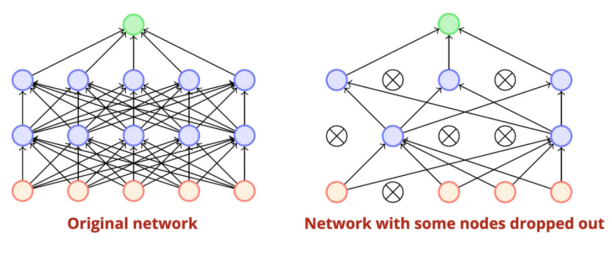
\includegraphics[width=0.8\textwidth]{img/1S-Rr9boTfKusUzETeKW6Mg.png}
\end{center}

In Pytorch, we simply need to introduce \texttt{nn.Dropout} layers specifying the rate at which to drop (i.e.~zero) units. Learning a neural network with dropout is usually slower than without dropout.

\emph{Source : \href{https://towardsdatascience.com/batch-normalization-and-dropout-in-neural-networks-explained-with-pytorch-47d7a8459bcd}{here}}

\textbf{2. High level description of your architechture}

We read many articles including the \href{https://www.kaggle.com/c/digit-recognizer/discussion/61480}{one} recommanded by this subject or \href{https://github.com/jeremyfix/deeplearning-lectures/blob/master/LabsSolutions/00-pytorch-FashionMNIST/models.py}{this one} and implemented \textbf{3 different architectures}, still on two epochs (using more epochs was too long to compute). See the codes in annex \ref{annexe:annexe1}.

\begin{enumerate}
\def\labelenumi{\arabic{enumi}.}
\tightlist
\item
  For the first architecture \texttt{ConvNet2}, we simply implementes the previous architecture \texttt{ConvNet} but we add a 50 \% probability dropout before the penultimate linear layer. The forward pass does not change.
\end{enumerate}

\textbf{\faArrowCircleRight{} The accuracy of \texttt{ConvNet2} is the same as the previous model (98,3 \% which is still very high) and thus does not improve the model. However, the model is slower because, as we said before, a neural network with dropout is usually slower.}

\begin{enumerate}
\def\labelenumi{\arabic{enumi}.}
\setcounter{enumi}{1}
\tightlist
\item
  For the second architecture \texttt{ConvNet3}, we use a more complicated network. Instead of using only 1 Conv2d-ReLU-MaxPool2d sequence, we use 3 of them. Then, we use 2 Linear-ReLU sequences instead of 1 and use before them a 50 \% probability dropout (as in \texttt{ConvNet3}). We also include a dropout in the forward pass. The more precise architecture is:

  \begin{itemize}
  \tightlist
  \item
    The input layer
  \item
    3 consecutive blocks with Conv(5×5, strides=1, padding=2)-Relu-MaxPooling(2×2, strides=2). It takes 16 filters for the first Conv layer, 32 filters for the second and 64 for the third one.
  \item
    Two dropout-linear-relu blocks of size 128 and 256, with 0.5 dropout probability
  \item
    One dense layer with 10 units (linear but softmax is then embedded in the loss function).
  \end{itemize}
\end{enumerate}

\textbf{\faArrowCircleRight{} We notice a real improvement in the accuracy of the model which is now 98,9 \% for \texttt{ConvNet3}. However, the model was slow to compute (around 30 min. on our computer for only 2 epochs).}

\begin{enumerate}
\def\labelenumi{\arabic{enumi}.}
\setcounter{enumi}{2}
\item
  Finally, for our third and last architecture, we use a very complex architecture, using not only \texttt{Conv2d}, \texttt{ReLu} and \texttt{MaxPool2d} layers but also \textbf{\texttt{BatchNorm2d}} and \textbf{\texttt{AvgPool2d}} in addition to Droupout:

  \begin{itemize}
  \tightlist
  \item
    \texttt{BatchNorm2d} applies Batch Normalization as described in \href{https://arxiv.org/abs/1502.03167}{this paper}. The fact that the parameters of the previous layers change changes the distribution of each layer's inputs and slows down the training. The goal is here to accelerate deep network training by reducing internal covariate shift.
  \item
    \texttt{AvgPool2d} applies an average pooling over an input signal composed of several input planes. Here, with global average pooling, we basically average pooling with a kernel of the same size (width,height) as the feature map.
  \end{itemize}

  If 64C3s1 denotes a convolutional layer with 64 kernels, of size 3×3, with stride 1, with zero padding, the precise architecture can be described as:

  \begin{itemize}
  \tightlist
  \item
    The input layer
  \item
    64C3s1-BatchNorm-Relu-64C3s1-BatchNorm-Relu - MaxPool2s2
  \item
    Droupout 40\% - 128C3s1-BatchNorm-Relu-128C3s1-BatchNorm-Relu - MaxPool2s2
  \item
    Droupout 40\% - 256C3s1-BatchNorm-Relu-256C3s1-BatchNorm-Relu - GlobalAverage(kernel size of 7)
  \item
    One dense layer with 10 units (linear but softmax is then embedded in the loss function).
  \end{itemize}

  Indeed, it is recently suggested in the litterature to use small convolutional kernels (3×3 or 5×5) because it leads to less parameters (and more non linearity). The number of filters is usually increased as we go deeper in the network (because we expect the low level layers to extract basic features that are combined in the deeper layers). Finally, Lin, Chen, \& Yan, 2013 suggested that we can completly remove the final fully connected layers and replace them by global average pooling. The network is thus less likely to overfit and you end up with much less parameters for a network of a given depth (this is the fully connected layers that usually contain most of your parameters).
\end{enumerate}

\textbf{\faArrowCircleRight{} We noticed another improvement in the accuracy of the model which is now 99,1 \% for \texttt{ConvNet4} but it took 40 minutes for 2 epochs.}

\begin{Shaded}
\begin{Highlighting}[]
\NormalTok{net }\OperatorTok{=}\NormalTok{ ConvNet4() }\CommentTok{#test the model of our choice ConvNetX (2 to 5)}

\CommentTok{# Loss and optimizer}
\NormalTok{criterion }\OperatorTok{=}\NormalTok{ nn.CrossEntropyLoss()}
\NormalTok{optimizer }\OperatorTok{=}\NormalTok{ torch.optim.Adam(net.parameters(), lr}\OperatorTok{=}\NormalTok{lr)}

\ControlFlowTok{for}\NormalTok{ epoch }\KeywordTok{in} \BuiltInTok{range}\NormalTok{(num_epochs):}
    
    \CommentTok{# makes one pass over the train data and updates weights}
\NormalTok{    train(net, trainloader, criterion, optimizer, epoch, num_epochs)}

    \CommentTok{# makes one pass over validation data and provides validation statistics}
\NormalTok{    val_loss, val_acc }\OperatorTok{=}\NormalTok{ validation(net, valloader, criterion)}
    
\end{Highlighting}
\end{Shaded}

\begin{Shaded}
\begin{Highlighting}[]
\NormalTok{test_loss, test_acc }\OperatorTok{=}\NormalTok{ validation(net, testloader, criterion)}
\BuiltInTok{print}\NormalTok{(}\SpecialStringTok{f'Test accuracy: }\SpecialCharTok{\{}\NormalTok{test_acc}\SpecialCharTok{\}}\SpecialStringTok{ | Test loss: }\SpecialCharTok{\{}\NormalTok{test_loss}\SpecialCharTok{\}}\SpecialStringTok{'}\NormalTok{)}
\end{Highlighting}
\end{Shaded}

\begin{verbatim}
Test accuracy: 0.9912 | Test loss: 0.027332775755273177
\end{verbatim}

\clearpage

\newpage

\hypertarget{appendix-appendix}{%
\appendix}


\addtocontents{toc}{\protect\setcounter{tocdepth}{1}}
\setcounter{page}{0}
\pagenumbering{roman}

\hypertarget{annexe:annexe1}{%
\section{Code of Problem 2}\label{annexe:annexe1}}

\begin{Shaded}
\begin{Highlighting}[]
\KeywordTok{class}\NormalTok{ ConvNet2(nn.Module):}
    \KeywordTok{def} \FunctionTok{__init__}\NormalTok{(}\VariableTok{self}\NormalTok{):}
        \BuiltInTok{super}\NormalTok{().}\FunctionTok{__init__}\NormalTok{()}
        \VariableTok{self}\NormalTok{.layer1 }\OperatorTok{=}\NormalTok{ nn.Sequential(}
\NormalTok{            nn.Conv2d(}\DecValTok{1}\NormalTok{, }\DecValTok{8}\NormalTok{, kernel_size}\OperatorTok{=}\DecValTok{5}\NormalTok{, stride}\OperatorTok{=}\NormalTok{[}\DecValTok{1}\NormalTok{, }\DecValTok{1}\NormalTok{], padding}\OperatorTok{=}\DecValTok{2}\NormalTok{),}
\NormalTok{            nn.ReLU(),}
\NormalTok{            nn.MaxPool2d(kernel_size}\OperatorTok{=}\DecValTok{2}\NormalTok{, stride}\OperatorTok{=}\DecValTok{2}\NormalTok{))}
        
        \VariableTok{self}\NormalTok{.classifier }\OperatorTok{=}\NormalTok{ nn.Sequential(}
\NormalTok{            nn.Dropout(}\FloatTok{0.5}\NormalTok{), }\CommentTok{#NEW DROPOUT = 50 % probability }
\NormalTok{            nn.Linear(}\DecValTok{14} \OperatorTok{*} \DecValTok{14} \OperatorTok{*} \DecValTok{8}\NormalTok{, }\DecValTok{500}\NormalTok{),}
\NormalTok{            nn.ReLU(),}
\NormalTok{            nn.Linear(}\DecValTok{500}\NormalTok{, }\DecValTok{10}\NormalTok{)}
\NormalTok{        )}
        
    \KeywordTok{def}\NormalTok{ forward(}\VariableTok{self}\NormalTok{, x):}
\NormalTok{        out }\OperatorTok{=} \VariableTok{self}\NormalTok{.layer1(x)}
\NormalTok{        out }\OperatorTok{=}\NormalTok{ out.reshape(out.size(}\DecValTok{0}\NormalTok{), }\DecValTok{-1}\NormalTok{)}
\NormalTok{        out }\OperatorTok{=} \VariableTok{self}\NormalTok{.classifier(out)}
        \ControlFlowTok{return}\NormalTok{ out}
\end{Highlighting}
\end{Shaded}

\begin{Shaded}
\begin{Highlighting}[]
\KeywordTok{class}\NormalTok{ ConvNet3(nn.Module):}
    \KeywordTok{def} \FunctionTok{__init__}\NormalTok{(}\VariableTok{self}\NormalTok{):}
        \BuiltInTok{super}\NormalTok{().}\FunctionTok{__init__}\NormalTok{()}
        \VariableTok{self}\NormalTok{.layer1 }\OperatorTok{=}\NormalTok{ nn.Sequential( }\CommentTok{#more complicated network}
\NormalTok{            nn.Conv2d(}\DecValTok{1}\NormalTok{, }\DecValTok{16}\NormalTok{,kernel_size}\OperatorTok{=}\DecValTok{5}\NormalTok{,stride}\OperatorTok{=}\DecValTok{1}\NormalTok{,padding}\OperatorTok{=}\BuiltInTok{int}\NormalTok{((}\DecValTok{5-1}\NormalTok{)}\OperatorTok{/}\DecValTok{2}\NormalTok{), bias}\OperatorTok{=}\VariableTok{True}\NormalTok{),}
\NormalTok{            nn.ReLU(inplace}\OperatorTok{=}\VariableTok{True}\NormalTok{),}
\NormalTok{            nn.MaxPool2d(kernel_size}\OperatorTok{=}\DecValTok{2}\NormalTok{),}
\NormalTok{            nn.Conv2d(}\DecValTok{16}\NormalTok{, }\DecValTok{32}\NormalTok{,kernel_size}\OperatorTok{=}\DecValTok{5}\NormalTok{,stride}\OperatorTok{=}\DecValTok{1}\NormalTok{,padding}\OperatorTok{=}\BuiltInTok{int}\NormalTok{((}\DecValTok{5-1}\NormalTok{)}\OperatorTok{/}\DecValTok{2}\NormalTok{), bias}\OperatorTok{=}\VariableTok{True}\NormalTok{),}
\NormalTok{            nn.ReLU(inplace}\OperatorTok{=}\VariableTok{True}\NormalTok{),}
\NormalTok{            nn.MaxPool2d(kernel_size}\OperatorTok{=}\DecValTok{2}\NormalTok{),}
\NormalTok{            nn.Conv2d(}\DecValTok{32}\NormalTok{, }\DecValTok{64}\NormalTok{,kernel_size}\OperatorTok{=}\DecValTok{5}\NormalTok{,stride}\OperatorTok{=}\DecValTok{1}\NormalTok{,padding}\OperatorTok{=}\BuiltInTok{int}\NormalTok{((}\DecValTok{5-1}\NormalTok{)}\OperatorTok{/}\DecValTok{2}\NormalTok{), bias}\OperatorTok{=}\VariableTok{True}\NormalTok{),}
\NormalTok{            nn.ReLU(inplace}\OperatorTok{=}\VariableTok{True}\NormalTok{),}
\NormalTok{            nn.MaxPool2d(kernel_size}\OperatorTok{=}\DecValTok{2}\NormalTok{)}
\NormalTok{        )}
        
\NormalTok{        probe_tensor }\OperatorTok{=}\NormalTok{ torch.zeros((}\DecValTok{1}\NormalTok{,}\DecValTok{1}\NormalTok{,}\DecValTok{28}\NormalTok{,}\DecValTok{28}\NormalTok{))}
\NormalTok{        out_features }\OperatorTok{=} \VariableTok{self}\NormalTok{.layer1(probe_tensor).view(}\OperatorTok{-}\DecValTok{1}\NormalTok{)}
\NormalTok{        num_classes }\OperatorTok{=} \DecValTok{10} 
        
        \VariableTok{self}\NormalTok{.classifier }\OperatorTok{=}\NormalTok{ nn.Sequential(}
\NormalTok{            nn.Dropout(}\FloatTok{0.5}\NormalTok{),}
\NormalTok{            nn.Linear(out_features.shape[}\DecValTok{0}\NormalTok{], }\DecValTok{128}\NormalTok{),}
\NormalTok{            nn.ReLU(inplace}\OperatorTok{=}\VariableTok{True}\NormalTok{),}
\NormalTok{            nn.Dropout(}\FloatTok{0.5}\NormalTok{),}
\NormalTok{            nn.Linear(}\DecValTok{128}\NormalTok{, }\DecValTok{256}\NormalTok{),}
\NormalTok{            nn.ReLU(inplace}\OperatorTok{=}\VariableTok{True}\NormalTok{),}
\NormalTok{            nn.Linear(}\DecValTok{256}\NormalTok{, num_classes)}
\NormalTok{        )}
        
    \KeywordTok{def}\NormalTok{ forward(}\VariableTok{self}\NormalTok{, x):}
\NormalTok{        out }\OperatorTok{=} \VariableTok{self}\NormalTok{.layer1(x)}
\NormalTok{        out }\OperatorTok{=}\NormalTok{ out.reshape(out.size(}\DecValTok{0}\NormalTok{), }\DecValTok{-1}\NormalTok{)}
\NormalTok{        out }\OperatorTok{=} \VariableTok{self}\NormalTok{.classifier(out)}
        \ControlFlowTok{return}\NormalTok{ out}
    
    
\end{Highlighting}
\end{Shaded}

\begin{Shaded}
\begin{Highlighting}[]
\KeywordTok{def}\NormalTok{ batch_relu(in_channels, out_channels, ks):}
    \ControlFlowTok{return}\NormalTok{ [nn.Conv2d(in_channels, out_channels,}
\NormalTok{                  kernel_size}\OperatorTok{=}\NormalTok{ks,}
\NormalTok{                  stride}\OperatorTok{=}\DecValTok{1}\NormalTok{,}
\NormalTok{                  padding}\OperatorTok{=}\BuiltInTok{int}\NormalTok{((ks}\DecValTok{-1}\NormalTok{)}\OperatorTok{/}\DecValTok{2}\NormalTok{), bias}\OperatorTok{=}\VariableTok{True}\NormalTok{),}
\NormalTok{        nn.BatchNorm2d(out_channels),}
\NormalTok{        nn.ReLU(inplace}\OperatorTok{=}\VariableTok{True}\NormalTok{)]}
    
\KeywordTok{class}\NormalTok{ ConvNet4(nn.Module):}

    \KeywordTok{def} \FunctionTok{__init__}\NormalTok{(}\VariableTok{self}\NormalTok{):}
        \BuiltInTok{super}\NormalTok{().}\FunctionTok{__init__}\NormalTok{()}
\NormalTok{        num_classes }\OperatorTok{=} \DecValTok{10}
\NormalTok{        base_n }\OperatorTok{=} \DecValTok{64}
        \VariableTok{self}\NormalTok{.features }\OperatorTok{=}\NormalTok{ nn.Sequential(}
            \OperatorTok{*}\NormalTok{batch_relu(}\DecValTok{1}\NormalTok{, base_n, }\DecValTok{3}\NormalTok{),}
            \OperatorTok{*}\NormalTok{batch_relu(base_n, base_n, }\DecValTok{3}\NormalTok{),}
\NormalTok{            nn.MaxPool2d(kernel_size}\OperatorTok{=}\DecValTok{2}\NormalTok{),}
\NormalTok{            nn.Dropout(}\FloatTok{0.4}\NormalTok{),}
            \OperatorTok{*}\NormalTok{batch_relu(base_n, }\DecValTok{2}\OperatorTok{*}\NormalTok{base_n, }\DecValTok{3}\NormalTok{),}
            \OperatorTok{*}\NormalTok{batch_relu(}\DecValTok{2}\OperatorTok{*}\NormalTok{base_n, }\DecValTok{2}\OperatorTok{*}\NormalTok{base_n, }\DecValTok{3}\NormalTok{),}
\NormalTok{            nn.MaxPool2d(kernel_size}\OperatorTok{=}\DecValTok{2}\NormalTok{),}
\NormalTok{            nn.Dropout(}\FloatTok{0.4}\NormalTok{),}
            \OperatorTok{*}\NormalTok{batch_relu(}\DecValTok{2}\OperatorTok{*}\NormalTok{base_n, }\DecValTok{4}\OperatorTok{*}\NormalTok{base_n, }\DecValTok{3}\NormalTok{),}
            \OperatorTok{*}\NormalTok{batch_relu(}\DecValTok{4}\OperatorTok{*}\NormalTok{base_n, }\DecValTok{4}\OperatorTok{*}\NormalTok{base_n, }\DecValTok{3}\NormalTok{),}
\NormalTok{            nn.AvgPool2d(kernel_size}\OperatorTok{=}\DecValTok{7}\NormalTok{)}
\NormalTok{        )}

        \VariableTok{self}\NormalTok{.lin1 }\OperatorTok{=}\NormalTok{ nn.Linear(}\DecValTok{4}\OperatorTok{*}\NormalTok{base_n, num_classes)}

    \KeywordTok{def}\NormalTok{ forward(}\VariableTok{self}\NormalTok{, x):}
\NormalTok{        x  }\OperatorTok{=} \VariableTok{self}\NormalTok{.features(x)}
\NormalTok{        x }\OperatorTok{=}\NormalTok{ x.view(x.size()[}\DecValTok{0}\NormalTok{], }\DecValTok{-1}\NormalTok{)}
\NormalTok{        y }\OperatorTok{=} \VariableTok{self}\NormalTok{.lin1(nn.functional.dropout(x, }\FloatTok{0.5}\NormalTok{, }\VariableTok{self}\NormalTok{.training, inplace}\OperatorTok{=}\VariableTok{True}\NormalTok{))}
        \ControlFlowTok{return}\NormalTok{ y}
\end{Highlighting}
\end{Shaded}

\end{document}
